Пусть $K$ — евклидово кольцо. Тогда а) Алгоритм Евклида в $K$ остановится. б) Последний не нулевой элемент $r_n$ в алгоритме Евклида — делитель $a$ и $b$. в) Найдутся такие $x, y \in K$, что $r_n = ax + by$. г) Определим наибольший общий делитель $a$ и $b$ как делитель $a$ и $b$ максимальной нормы. Тогда $r_n$ — наибольший общий делитель

\Proof

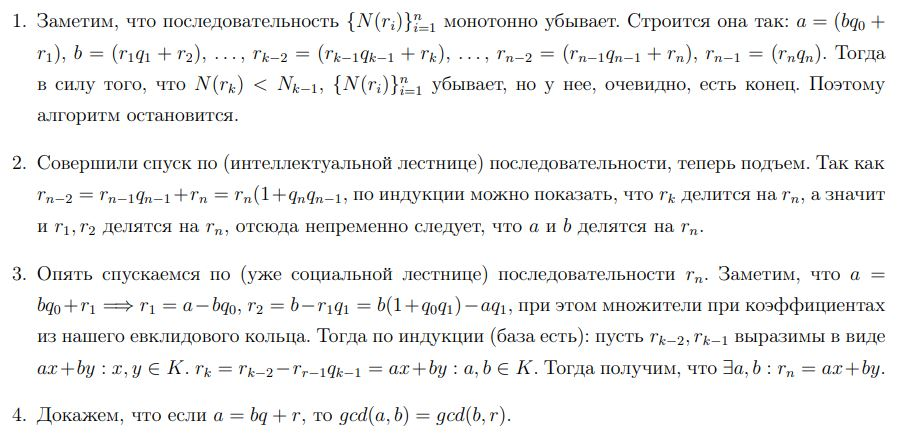
\includegraphics[scale=0.95]{images/4_11_1.JPG}

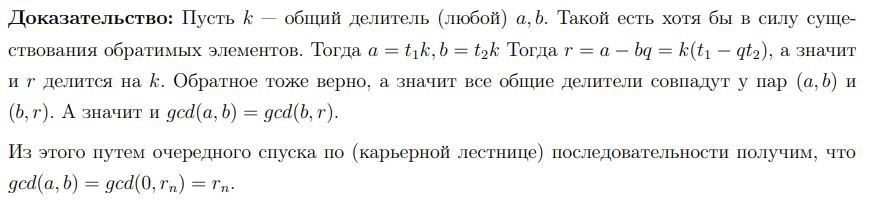
\includegraphics[scale=0.95]{images/4_11_2.JPG}

\EndProof